%
%  kant.six
%
%  Created by Mark Eli Kalderon on 2008-01-19.
%  Copyright (c) 2008 Mark Eli Kalderon. All rights reserved.
%
%  Beamer

% Definitions and macros
\newcommand{\change}{\textcolor{blue}{\textbf{CHANGE SLIDE}}}
\newcommand\myauthor{Mark Eli Kalderon} 
\newcommand\mytitle{Introduction to Moral Philosophy}
\newcommand\mysubtitle{Kant}
\newcommand\myinstitution{University College London}
\newcommand\myurl{http://markelikalderon.com/teaching}

% Packages specific to lecture notes
\mode<article>{
    \usepackage{palatino}
    \setjobnamebeamerversion{kant.six.beamer}
}


% Packages specific to beamer presentation
\mode<presentation>{
    \usetheme{Darmstadt}
    \setbeamercovered{transparent}
    \pgfdeclareimage[height=0.5cm]{university-logo}{../../graphics/logo_sml_blk}
    \logo{\pgfuseimage{university-logo}}
}

% Packages common to lecture notes and beamer presentation
\usepackage{pgf}
\usepackage{tikz}
\usepackage{hyperref}

\title{\mytitle}
\subtitle{\mysubtitle}

\author{\myauthor\\
\url{\myurl}}
\institute{\myinstitution}

% \date[Short Occasion] % (optional)
% {Date / Occasion}

\begin{document}

\frame{\maketitle}

\section{Introduction}\label{sec:introduction} % (fold)

\change\ Throughout the first two sections of the Groundwork, Kant repeatedly insists that his search for the moral law is \emph{conditional}: He merely assumes the existence the supreme principle of morality, and then seeks to establish that it has a certain character (in the first section, Kant argues that it can be represented by the Formula of Universal Law and in the second section Kant argues that it can be represented by the system of three formulas). In the third section, Kant discharges this assumptions by arguing that morality is not an illusion, that there is indeed a categorical imperative binding on rational beings. In the third section, Kant finally establishes the existence of the supreme principle of morality.

Kant’s deduction of the moral law is complex and difficult to interpret. Moreover, the argument he presents in the Groundwork was obviously unsatisfying to him at least by the time he wrote the Critique of Practical Reason three years later. There, Kant argued that the existence of the moral law admits of no deduction but is rather a self-evident fact of reason. Today’s discussion of Kant’s argument will not be drawn from a close reading of a single text but will be a deliberately simplified reconstruction that draws on ideas in the Groundwork that are representative of his moral thinking throughout the critical period. \change

\begin{frame}<presentation>[label=slide1]
    \frametitle{The Project of the Third Section}
        \begin{columns}
            \begin{column}{3cm}
                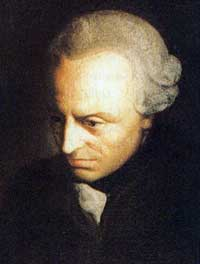
\includegraphics[height=4cm]{../../graphics/kant.jpg}
            \end{column}
            \begin{column}{7cm}
                \begin{itemize}
                    \item In the first two sections, Kant merely assumes the existence of the supreme principle of morality, and then argues that it must have a certain character, i.e. that it is represented by the system of three formulas.
                    \item In the third section, Kant discharges the assumption that there is a categorical imperative binding on rational beings, that the supreme principle of morality exists.
                \end{itemize}
            \end{column}
        \end{columns}
\end{frame}

% section introduction (end)

\section{The Deduction}\label{sec:the_deduction} % (fold)

The basis of Kant’s deduction of the moral law is what Henry Allison calls the ``Reciprocity Thesis''. Consider the following two claims:

\begin{itemize}
    \item \emph{Freedom}: The rational will is free.
    \item \emph{Morality}: The moral law is unconditionally valid for the rational will.
\end{itemize}

The \emph{Reciprocity Thesis} claims that \emph{Freedom} and \emph{Morality} are mutually entailing:

\begin{itemize}
    \item \emph{Reciprocity}: The rational will is free iff the moral law is unconditionally valid for the rational will.
\end{itemize}

Notice that \emph{Reciprocity} is really two claims in one:

\begin{itemize}
    \item \emph{Freedom Entails Morality}: If the rational will is free, then the moral law is unconditionally valid for the rational will.
    \item \emph{Morality Entails Freedom}: If the moral law is unconditionally valid for the rational will, then the rational will is free.
\end{itemize}


Whereas \emph{Reciprocity} is emphasized in the \emph{Critique of Practical Reason}, in the \emph{Groundwork}, Kant emphasizes \emph{Freedom Entails Morality}.

The argument of the third section of has two components:

\begin{enumerate}
    \item Kant provide an argument for \emph{Freedom Entails Morality}: If the rational will is free, then the moral law is unconditionally valid for the rational will.
    \item Kant argues that the freedom of the rational will is an indispensable presupposition of rational judgment
\end{enumerate}

Given these two claims, it follows that the moral law is unconditionally valid for the rational will. \change

\begin{frame}<presentation>[label=slide2]
    \frametitle{Freedom and Morality}
        \begin{columns}
            \begin{column}{3cm}
                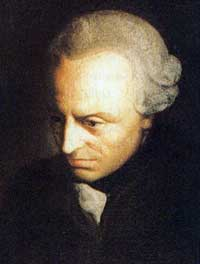
\includegraphics[height=4cm]{../../graphics/kant.jpg}
            \end{column}
            \begin{column}{7cm}
                \begin{itemize}
                    \item \alert{Freedom}: The rational will is free
                    \item \alert{Morality}: The moral law is unconditionally valid for the rational will
                    \item \alert{Freedom Entails Morality}: If the rational will is free, then the moral law is unconditionjally valid for the rational will
                \end{itemize}
            \end{column}
        \end{columns}
\end{frame}

Kant distinguishes several senses of freedom:
\begin{itemize}
    \item \emph{Transcendental freedom} is the capacity of a cause to produce a state spontaneously or ``from itself''. A transcendentally free cause is a ``first cause'', an ``unmoved mover'', one that can be effective independently of any prior cause.
    \item \emph{Practical Freedom} is the freedom that we attribute to ourselves as rational agents.
\end{itemize}
Kant’s central metaphysical contention in the Groundwork is that the will is practically free only if it is transcendentally free. Given this, we will focus exclusively on practical freedom. 

Practical freedom, in turn, has two senses:
\begin{itemize}
    \item A will is \emph{negatively free} if it acts independently of external causes determining how it acts.
    \item A will is \emph{positively free} if it has the power to determine itself in accordance with its own law.
\end{itemize}

\change

\begin{frame}<presentation>[label=slide3]
    \frametitle{The Varieties of Freedom}
        \begin{columns}
            \begin{column}{3cm}
                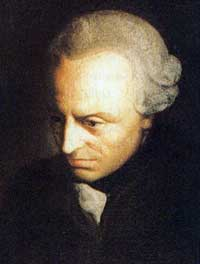
\includegraphics[height=4cm]{../../graphics/kant.jpg}
            \end{column}
            \begin{column}{7cm}
                \begin{itemize}
                    \item \emph{Transcendental freedom} is the capacity of a cause to produce a state spontaneously or ``from itself''. A transcendentally free cause is a ``first cause'', an ``unmoved mover'', one that can be effective independently of any prior cause.
                    \item \emph{Practical Freedom} is the freedom that we attribute to ourselves as rational agents.
                    \item A will is \emph{negatively free} if it acts independently of external causes determining how it acts.
                    \item A will is \emph{positively free} if it has the power to determine itself in accordance with its own law.
                \end{itemize}
            \end{column}
        \end{columns}
\end{frame}

Kant’s deduction of the moral law has two components. The first component is an argument for \emph{Freedom Entails Morality}: If the rational will is free, then the moral law is unconditionally valid for the rational will. Kant argues for Freedom  Morality on the grounds that freedom is a kind of causality and an analysis of what ``causality'' must mean in the case of freedom.

The key to understanding how the existence of the moral law might be deduced from the freedom of the will is Kant’s conception as freedom as a special kind of causality. If freedom is a special kind of causality then it must operate in accordance with laws. Just as natural causes operate in accordance with the laws of nature, so free causes must operate in accordance with the laws of freedom. That much, according to Kant, follows from the very concept of causality. The laws of freedom differ in one fundamentally important respect from the laws of nature. Natural causes act according to natural laws. However, a will not only acts according to laws but according to their representation. So the law of the free cause must be one that it represents to itself. In the case of the imperfectly rational will, which does not always act as reason directs, the law is represented as a principle according to which it ought to act. The laws of freedom are thus normative laws, they concern what ought to happen whereas natural laws concern what actually happens. 

This is not as odd as it might sound. Just as there are natural explanations, explanations based on natural law, there are, intuitively at least, normative explanations, explanations based on normative law. After all, we explain human action in terms of the norms they accept: A chess player only moves the bishop diagonally because of the rules of chess. In making grammatical utterances of English, speakers utter the words they do because of the rules of English grammar.

Normative explanations are appropriate to voluntary rational action because rational actions are by their very concept freely chosen and norm-guided. All intentional action are subject to normative explanation insofar as every intention to pursue an end requires subscribing to certain norms (such as the principles involved in means-end reasoning). \change

\begin{frame}<presentation>[label=slide4]
    \frametitle{Freedom as Causality}
        \begin{columns}
            \begin{column}{3cm}
                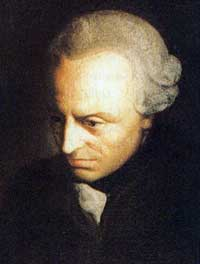
\includegraphics[height=4cm]{../../graphics/kant.jpg}
            \end{column}
            \begin{column}{7cm}
                \begin{itemize}
                    \item Just as \alert{natural causes} operate in accordance with \alert{the laws of nature}, so \alert{free causes} operate in accordance with \alert{the laws of freedom}
                    \item A will not only acts according to laws but according to their representation
                    \item Just as the laws of nature are unconditionally valid for empirical objects, so the laws of freedom are unconditionally valid for rational beings
                \end{itemize}
            \end{column}
        \end{columns}
\end{frame}

Kant argues that given what causality means in the case of freedom, the operation of a free cause must be in accordance with an unconditional and self-given normative law. In the Second Section, Kant argued that according to the Formula of Autonomy the moral law just is an unconditional self-given normative law. Therefore if the will is free the moral law is valid for it. Kant’s argument for the first premise can be represented as follows:

\begin{itemize}
	\item A free cause acts in accordance with an unconditional and self-given normative law.
	\item The moral law is an unconditional and self-given normative law.
	\item If the rational will is free, the moral law is unconditionally valid for it.
\end{itemize}

To complete the deduction of the moral law, Kant must discharge the antecedent of the conditional by showing that we have reason to believe that the rational will is free.

Kant does not think that the freedom of the will can be theoretically demonstrated. There is no question then of providing a deductive argument for it that is both sound and convincing. Indeed Kant seems to think not only that the freedom of the will cannot be theoretically demonstrated but that it cannot be theoretically cognized at all. 

% In the \emph{Critique of Pure Reason} Kant argues that the idea of freedom is transcendent in the sense that no experience can be adequate to it. From this he concludes two things. First that freedom cannot be attributed to the will as an object of experience and second that no experience can ever show that the will is not free. But the transcendental idealist metaphysics tends to distract from what is important to Kant’s deduction of the moral law. We will understsand the deduction better if we focus of the (quite unmetaphysical) way in which Kant considers freedom in the deduction itself.

In the \emph{Groundwork} Kant claims that ``freedom must be presupposed as a property of the will of all rational beings'' (G 4:447). Freedom is not being proved theoretically, but is claimed to be a presupposition of taking the practical standpoint at all---which we must unavoidably do, even when we are engaged in theoretical inquiry. \change

\begin{frame}<presentation>[label=slide5]
    \frametitle{The Argument for Freedom Entails Morality}
        \begin{columns}
            \begin{column}{3cm}
                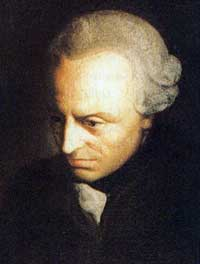
\includegraphics[height=4cm]{../../graphics/kant.jpg}
            \end{column}
            \begin{column}{7cm}
                \begin{itemize}
                    \item The free cause acts in accordance with an unconditional and self-given noramtive law
                    \item By the \alert{Formula of Autonomy}, the moral law just is an unconditional and self-given normative law
                    \item If the rational will is free, the moral law is unconditionally valid for it
                \end{itemize}
            \end{column}
        \end{columns}
\end{frame}

Kant writes:
\begin{quote}
    Now, one cannot possibly think of a reason that would consciously receive direction from another quarter with respect to its judgments since the subject would then attribute the determination of his judgment not to reason but to impulse. Reason must regard itself as the author of its principles independently of alien influences; consequently, as practical reason or as the will of a rational being must be regarded of itself as free. (G 4:448)
\end{quote}
Notice that these remarks, focusing not on \emph{actions} but only on \emph{judgments} concern the way in which we must regard ourselves in making judgments of any sort, even wholly theoretical ones. If even there we must regard ourselves as free, then there is no room in any sort of understanding of ourselves for a conception of ourselves as other than free.

Kant holds that we must think of ourselves as free in all our rational judgments in the sense that we must regard our judgments as actions we perform under norms. Because Kant is thinking of freedom as action under a norm, Kant must understand freedom to mean something other than arbitrariness but rather something close to its opposite. If I judge that q based on the evidence that \emph{if p then q} and \emph{p}, then I cannot regard this as a rational judgment on my part only if I am prepared to give it a normative explanation, by viewing it as proceeding from my correct application of the logical rule of modus ponens regarded as a normative principle which I simply as a rational being recognize as valid and impose on my own judgments. Thus to say that judgment is the exercise of free agency in this sense is precisely not to say that I may judge any way I please. On the contrary my judgment can go contrary to the norm only if it involves a failure or a mistake. If I think of my judgment as prompted by some conscious cause external to my free and rational norm guided activity (for example, if I see it as prompted by fear of what my logic teacher will do to me if I don’t give the answer of which I know he appreoves) then to that extent I cease to regard it as a judgment which is rational by the standard of the relvant norms. If my fear of my logic teacher prompts me to give the right answers, that will be because those happen to be the ones he wants; but the rightness of my judgment would be only contingently the result of anyone’s applying rational norms (and the rationality of my judgments would have to be ascribed to my logic teacher and not me). The verdict would be the same if I came to regard my judgment as the result of some unconscious process (of neurotic compulsion or posthypnotic suggestion) whose results accord only contingently with the rules of logical inference. Not all of my reasoning need be entirely conscious and explicit, but to regard them as successful reasoning, they must be regarded as the result of my freely (though perhaps habitually and unreflectively) following rational norms.

How is this argument relevant to moral freedom? Kant’s idea seems to be that the capacity that we ascribe to ourselves in thinking of ourselves as subject to moral obligations is the same kind as that we ascribe to ourselves in thinking of ourselves as judging according to rational norms, so that if we cannot intelligibly doubt that we have such a capacity in one case, we cannot intelligibly doubt it in the other. We cannot intelligibly doubt that we judge according to rational norms. Moreover rational norms make unconditional demands on us. If we accept the validity of modus ponens we don’t accept it conditional on some advantage it affords. On the contrary we accept it as unconditionally necessary to preserve the truth of our judgments.

To understand myself as capable of judging is to assume that I am free in precisely in the sense meant in \emph{Freedom Entails Morality} and to understand myself as judging rationally is therefore to presuppose that the rational will is free. Since we have already established \emph{Freedom Entails Morality}, all those who think of themselves as making rational judgments already presuppose something that commits them to the moral law being unconditional valid for all rational beings. \change

\begin{frame}<presentation>[label=slide6]
    \frametitle{Freedom and Judgment}
        \begin{columns}
            \begin{column}{3cm}
                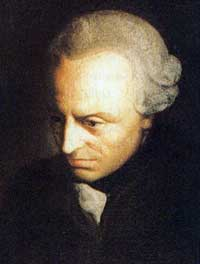
\includegraphics[height=4cm]{../../graphics/kant.jpg}
            \end{column}
            \begin{column}{7cm}
                Now, one cannot possibly think of a reason that would consciously receive direction from another quarter with respect to its judgments since the subject would then attribute the determination of his judgment not to reason but to impulse. Reason must regard itself as the author of its principles independently of alien influences; consequently, as practical reason or as the will of a rational being must be regarded of itself as free. (G 4:448)
            \end{column}
        \end{columns}
\end{frame}

Let’s consider one application of this idea. Let a \emph{fatalist} be someone who denies practical freedom understood as causality according to normative law. The fatalist must regard his own acts of judgments solely as necessary effects of natural laws, denying that they can be correctly explained by reference to reasons or normative rules of inference (such as modus ponens). 

If fatalism is to be an interesting position, then the fatalist must be prepared to give arguments for fatalism, to assert fatalism on the basis of arguments, and expect those to whom she gives arguments to be convinced of fatalism on the basis of them. Yet fatalism itself says that all judgements (including the fatalist’s judgement that the rational will is not free) are to be explained solely by reference to natural laws and can never be explained by reference to normative laws such as the laws of reasoning. Fatalism, itself, therefore undermines the fatalist’s claim that he and those he tries to persuade of fatalism can hold fatalism on rational grounds. \change

\begin{frame}<presentation>[label=slide7]
    \frametitle{Fatalism}
        \begin{columns}
            \begin{column}{3cm}
                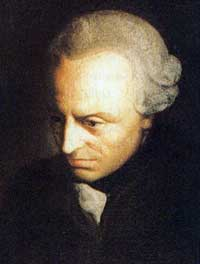
\includegraphics[height=4cm]{../../graphics/kant.jpg}
            \end{column}
            \begin{column}{7cm}
                \begin{itemize}
                    \item \alert{Fatalism}: The rational will is not free
                    \item The fatalist must hold fatalism on the basis of reasons
                    \item The fatalist claims that all judgments, including the judgment that the rational will is not free, are explained solely in terms of natural laws and cannot be explained in terms of normative laws
                    \item Fatalism undermines the fatalist's claim that he holds fatalism on the basis of reasons
                \end{itemize}
            \end{column}
        \end{columns}
\end{frame}

According to Kant, we must presuppose that we are free if we regard ourselves as rational. Freedom is a kind of causality. It follows from the concept of causality that the operation of freedom is law governed just like the operation of natural causes. The laws of freedom are unconditionally valid for all rational beings, just like the laws of nature are unconditionally valid for all natural beings. However, unlike natural causes, freedom operates under a representation of a law that it imposes on itself. So in presupposing that we are free, we presuppose that our will is governed by a law unconditionally valid for all rational beings and that in acting freely we act under a representation of such a law that we impose upon ourselves. But this is just the moral law as represented by the Formula of Autonomy.

Thus according to Kant, our presupposition that we are free analytically entails that the moral law is unconditionally binding on the rational will. This should be sufficient for the avowed purpose of Section Three, to establish the existence of the moral law. For if we must presuppose that we are free, and this entails that the moral law is unconditionally valid for all rational beings, then we must presuppose that the moral law exists. However, Kant expresses dissatisfaction with only establishing this much. These reflections may establish that we must presuppose that the moral law exists but they do not by themselves establish our interest in the moral law. They may establish that we must presuppose that we are subject to the moral law if we regard ourselves as rational, but it doesn’t reveal the nature of the interest we would take in the moral law in acting from duty.

Recall the distinction Kant draws between acting in accordance with duty and acting from duty. Acting in accordance with duty is merely fulfilling the requirements of duty regardless of motivation. Acting from duty is to be motivated in a particular way to act in accordance with duty, by recognizing that it is one’s duty. Acting from duty thus involves acting on a representation of duty, a representation of at least some aspect of the moral law. Moreover a representation of the moral law can motivate us to do our duty without supporting inclination or even in the face of conflicting inclination. According to Kant whenever we act we act from some interest. When we act from inclination, inclination is the grounds of our interest in the represented object of inclination. But what is the grounds of our interest in the represented moral law when we act from duty? Consider the case where we are motivated to do our duty in the face of contrary inclination. Suppose you want to do something. If upon reflection you decide that it would be wrong of you to do that thing, this might motivate you to refrain from doing that thing even if your happiness depended upon it. If you do act from duty the thought that you cannot will that your maxim be a universal law must motivate you to refrain from furthering your happiness. In order to be so motivated we would have to assign a kind of value to autonomy and to ourselves insofar as we are capably of acting autonomously that is incomparably greater than the object of our inclination. A value that our happiness in comparison ``is to be held as nothing'' The argument presented so far does not show us how this is possible. It may establish that we can be motivated in this way (that’s why it suffices for the exitence of the moral law) but it doesn’t explain the intelligibility of being so motivated. The second argument of the third section is supposed to explaint the interest we display in the moral law that we impose upon ourselves. \change

\begin{frame}<presentation>[label=slide8]
    \frametitle{From Practical Freedom to Transcendental Freedom}
        \begin{columns}
            \begin{column}{3cm}
                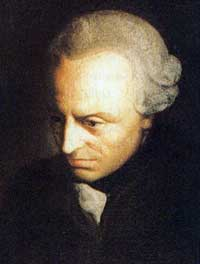
\includegraphics[height=4cm]{../../graphics/kant.jpg}
            \end{column}
            \begin{column}{7cm}
                \begin{itemize}
                    \item While the argument establishes that we can be motivated to act from the moral law, it does not yet explain our interest in it
                    \item In order to explain our interest in the moral law, Kant needs to appeal to more than just \alert{practical freedom}, he needs to appeal to \alert{transcendental freedom}
                \end{itemize}
            \end{column}
        \end{columns}
\end{frame}

Let’s begin with a distinction that Kant draws between the noumenal and phenomenal worlds. These aren’t literally worlds, but conceptions of the word. The noumenal world is the conception of the world as it is in itself. The phenomenal world is the conception of the wolrd as it appears to us. These two conceptions of the world arise from reflecting on the cognitive relations we bear to the world. When we know something on the basis of experience it appears a certain way to us. The phenomenal world is just the world conceived as it appears to us in experience. We are passive in the face of the world of appearance and so naturally think that there are things that stand behind these appearances and generate them. So while we can only know the phenomenal world, the world of sense experience, we can think of the noumenal world, the way the world is in and of itself. These are distinct epistemic perspectives on the world: as it is given to us in sense experience and how we think it must be independently of us. The phenomenal world is the world of sense and the noumenal world is the world of understanding.

Kant applies this distinction in resolving the apparent conflict between free will and determininism. 
Let’s begin with the conflict. According to determinism, every event is the effect of some cause. But the law that every effect has a cause is inconsistent with there being uncaused causes---causes which are the effects of no other cause. But this is how we must conceive of the will if it is to be genuinely free. In this way determinism seems to be inconsitent with the will being free.

Kant reconciles free will and determinism by applying the distinction between the phenomenal and noumenal worlds. According to Kant, the operation of empirical causation is limited to the phenomenal world. Thus the law every effect has a cause is a law that governs how things must appear to us. Causal law applies to the world insofar as it is knowable on the basis of expereince, not necessarily to how the world really is independently of experience. In thinking of the free will as an uncaused causer we are thinking of how the will must be and not how the will appears to us. Free will is not after all incompatible with determinism. Determinism applies to the phenomenal world, the world of appearances, while the conception of the will as free applies to how the will must be in itself and not ncessarily to how it appears to us.
Notice that we cannot know that we are free. Knowledge is limited to the world of appearance. But that does not mean that there are no grounds for thinking that we are free. \change

\begin{frame}<presentation>[label=slide9]
    \frametitle{Free Will and Determinism}
        \begin{columns}
            \begin{column}{3cm}
                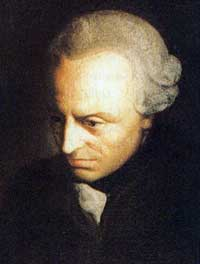
\includegraphics[height=4cm]{../../graphics/kant.jpg}
            \end{column}
            \begin{column}{7cm}
                \begin{itemize}
                    \item The law that every event is the effect of some cause applies only to the phenomenal world
                    \item The conception of the will as an uncaused causer is a conception of how the will must be in itself if it is to be free---it applies only to the noumenal world
                \end{itemize}
            \end{column}
        \end{columns}
\end{frame}

The distinction between the phenomenal and noumenal worlds applies to ourselves as well. These are two epistemic perspectives that we may adopt otwards ourselves. Thus Kant writes that there are ``two standpoints from which we can regard himself and cognize laws for the use of his powers and consequently for all of his actions'' When we view ourselves as members of the sensible or phenomenal world we regard ourself and everything about ourself including inner appearances such as our thoughts and choices as parts of the sensible world and so as governed by the causal laws that govern the sensible world. But if we regard ourselves as rational beings we view ourselves as the author of our thoughts and choices. That is we regard ourselves as the first and ultimate cause of these inner appearances. Insofar as we do we think of ourselves as members of the noumenal world, the world of understanding. It is because we can think of ourselves as members of the world of understanding that we can think of ourselves as free and so as capable of autonomous action. 
We must see ouselves as being memebers of the phenomenal and noumenal worlds as being memebers of the world of sense and the world of understanding. Insofar as we are members of the world of sense, our actions are governed by the law of cause and effect. Insofar as we are members of the world of understanding, our will is free and we governed only by laws that we give ourselves. According to Kant the world of understanding contains the ground of the world of sense and so too of its laws. So as members of the world of understanding we give laws to ourself as members of the world of sense. If the moral law is conceived in this way, as a law that we as members of the world of understanding give to ourselves as members of the sensible world, only then is it intelligible that we could act from a representation of that law in the face of conflicting duty. Acting from duty expresses respect for the dignity of our noumenal nature as transcendentally free rational beings.

\begin{frame}<presentation>[label=slide10]
    \frametitle{The Final Derivation}
        \begin{columns}
            \begin{column}{3cm}
                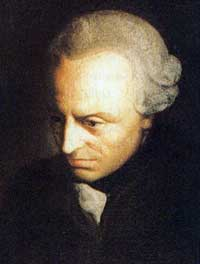
\includegraphics[height=4cm]{../../graphics/kant.jpg}
            \end{column}
            \begin{column}{7cm}
                \begin{itemize}
                    \item In viewing ourselves as members of the noumenal world, we must think of ourselves as giving laws to ourselves as members of the phenomenal world
                    \item It is only form the perspective of our noumenal nature that acting from the moral law is intelligible and of interest
                \end{itemize}
            \end{column}
        \end{columns}
\end{frame}

% section the_deduction (end)

\section*{Summary}

\end{document}
